\newpage

\section{Diagrammi di Fase}

Definiamo \textbf{\textbf{fase}} quella porzione del sistema che presenta composizione omogenea e proprietà costanti. Se a livello microscopico osserviamo che la definizione non è più corretta si parla di \textbf{\textit{microcostituenti}} (esistono casi in cui si ha una microstruttura formata da due fasi differenti, come ad esempio la perlite).
I diagrammi permettono di studiare il materiale in esame:
\begin{itemize}
    \item Permette di determinare la solubilità di un materiale in un altro in funzione della temperatura.
    \item Permette di sapere i range di temperatura per cui è favorita una forma rispetto un'altra
    \item Permette di conoscere le temperature di fusione dei vari componenti.
\end{itemize}
Vengono ottenuti raccogliendo le curve di raffreddamento di una sostanza a diverse pressioni o di un miscuglio a diversi rapporti di concentrazione.
Le curve di raffreddamento presentano pendenze diverse in base alla capacità termica che a sua volta dipende dallo stato fisico della materia e dalla composizione. Durante le transizioni di fase si ha un plateau nella temperatura nel caso di sostanze pure. Un'importante regola che viene sempre seguita è quella delle fasi di Gibbs che stabilisce il numero di gradi di libertà $f$ di un sistema formato da n componenti e p fasi:
\begin{equation}
    f = 2+n-p
\end{equation}
Tenendo la pressione costante il numero di gradi di libertà è ridotto di 1.

\subsection{Soluzioni a due componenti}

Le soluzioni sono miscugli omogenei (sia che siano formate di solidi che di liquidi) che presentano una singola fase.
Due o più sostanze tendono a formare una soluzione stabile quando questa è energeticamente favorita:
\begin{equation}
    \Delta G_{mix}=G_{ab}-(G_a+G_b)<0
\end{equation}
Una soluzione di due sostanze A e B si dice ideale se:
\begin{itemize}
    \item Le particelle dei due costituenti hanno uguale dimensione.
    \item L'energia di interazione è la stessa per le coppie A-A, A-B e B-B.
\end{itemize}
In condizioni ideali l'energia libera di mescolamento è pertanto dovuta solo a motivi entropici (le condizioni precedenti assicurano che l'entalpia di mescolamento sia nulla).
\begin{equation}
    \Delta G_{mix}=-RT(n_a \ln(\chi_a)+n_b \ln(\chi_b))
\end{equation}
E quindi dovrebbero sempre essere energeticamente favorite e l'aumento di entropia risulta la driving force del processo.
In generale queste assunzioni non sono sempre vere, dunque si applica un modello che permette una trattazione più complessa ma ancora gestibile, la teoria delle soluzioni regolari, che tiene conto delle interazioni tra particelle differenti tramite un termine aggiuntico della forma:
\begin{equation}
    \Delta G^{xs}_{mix}=a_{AB}\chi_A\chi_B
\end{equation}
Quando si ha un valore di $\Delta H^{mix}\neq 0$ abbiamo la formazione di un azeotropo di massimo o minimo (a seconda del segno, se positivo si ha un minimo; in caso contrario un massimo).
\begin{figure}[h]
    \centering
    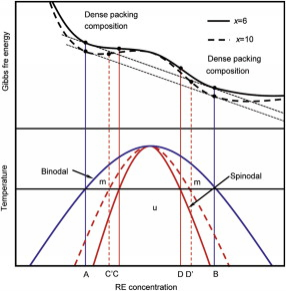
\includegraphics[width=6cm]{Diagrammi di fase/binodal.png}
    \caption{Caption}
    \label{binodal}
\end{figure}
In genere ad una data temperatura potremmo avere una fase molto più stabile dell'altra oppure una situazione in cui si hanno due minimi come in Fig \ref{binodal}. In questo caso per concentrazioni comprese tra i due punti di flesso (detti \textbf{\textit{punti spinodali}}) è favorita la decomposizione a dare due fasi distinte, mentre se la concentrazione si trova tra il punto \textbf{\textit{binodale}} (quello individuato dalla tangente alla curva) e quello spinodale si ha una fase metastabile in quanto la separazione in due fasi non è favorita (per convincersi di questi differenti trend è sufficiente ricordare la definizione di funzione concava/convessa).

\subsection{Leghe binarie}

\epigraph{[...] le temperatura di transizione (dette \textbf{\textit{incongruenti}}) non risultano un valore preciso ma un intervallo di temperatura}{\textit{Leonardo Sabattini}, I edizione}

Perchè si formino delle soluzioni completamente miscibili dobbiamo avere il soddisfacimento delle regole di Hume-Rothery cioè atomi con dimensioni simili stessa valenza ed elettronegatività e stessa struttura cristallina. In questo caso è possibile ottenere delle miscele con solubilità completa in tutto l'intervallo di composizione. Un esempio è riportato in Fig \ref{diagramma_tot_misc}.
\begin{figure}[h]
    \centering
    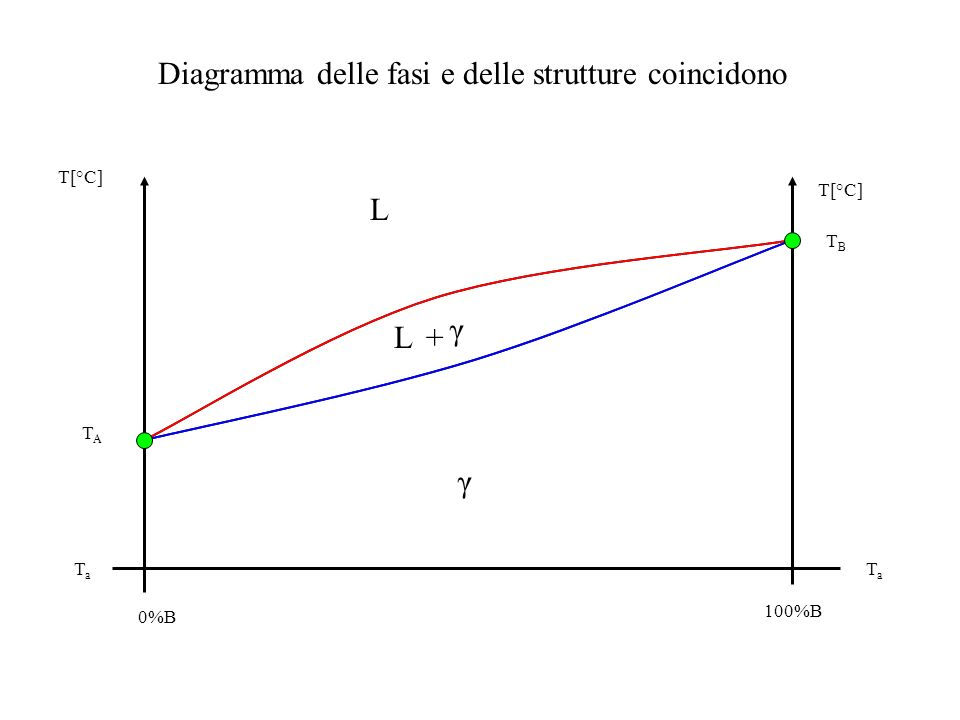
\includegraphics[width=8cm]{Diagrammi di fase/diagramma_stato1.jpg}
    \caption{Diagramma di stato di un sistema binario totalmente miscibile.}
    \label{diagramma_tot_misc}
\end{figure}

Un aspetto interessante delle soluzioni sia solide che liquide è che in generale la temperatura di transizione non assume un valore preciso, ma il processo avviene in un intervallo di temperatura. In generale, diminuendo la temperatura si arriverà nella zona intermedia in cui sono presenti sia la fase liquida che quella solida.
Se ci si trova in un punto all'interno di questa zona sono presenti due fasi ($L+\gamma$) in proporzione definita dalla lunghezza dei segmenti isotermi che congiungono il punto alle curve (vedasi \textit{regola della leva}). La fase liquida risulta arricchita del componente bassofondente mentre la fase solida risulta maggiormente arricchita della specie altofondente. Diminuendo ancora la temperatura tutta la fase liquida solidifica.\\
Queste curve sono ottenute sempre considerando casi in cui si ha il tempo necessario per permettere l'instaurarsi dell'equilibrio ed è lecito domandarsi cosa accade quando queste condizioni non valgono, in particolar modo in fase solida dove la diffusione ha minor peso. Il primo cristallita che si forma avrà composizione diversa dal liquido iniziale (ricco dell'altofondente), gli strati successivi saranno via via più poveri della specie altofondente poiché il raffreddamento repentino non riesce ad equilibrarsi e cambiare la sua composizione. L'ultimo guscio avrà composizione dell'altofondente minore della soluzione iniziale. Questo processo può generare fenomeni non voluti in quanto i bordi di grano risultano essere composti di fasi che fondono a T minore (essendo più ricchi nella fase bassofondente), e questo può causare problemi quando si lavora ad elevate temperature. Per ottenere nuovamente un sistema omogeneo non occorre sempre rifondere l'intero manufatto, ma è comunque necessario aumentare la temperatura.

\subsection{Insolubilità}

Nel caso di un sistema binario A-B solubili nello stato liquido ma insolubili nello stato solido si ha una legge del tipo:
\begin{equation}
    \chi_B=\frac{\Delta H_A(T_{m,A}-T_m)}{R \ T^2_{m,A}}
\end{equation}
Dove $T_{m,A}$ è la temperatura a cui inizia la solidificazione. Una legge analoga vale anche considerando $\chi_A$. Si osserva dunque che la temperatura di fusione in questo caso è sempre minore a quella della sostanza pura ed esiste un punto in cui si ha il passaggio diretto dalla fase solida A+B alla fase liquida, come mostrato in fig. \ref{eutettico}. Questa particolare composizione è detta \textit{\textbf{composizione eutettica}}; la temperatura a cui avviene la transizione, detta \textbf{\textit{temperatura eutettica}}, rappresenta la minima temperatura a cui può esistere la fase liquida.

\begin{figure}[h]
\begin{minipage}[b]{0.5\linewidth}
\centering
    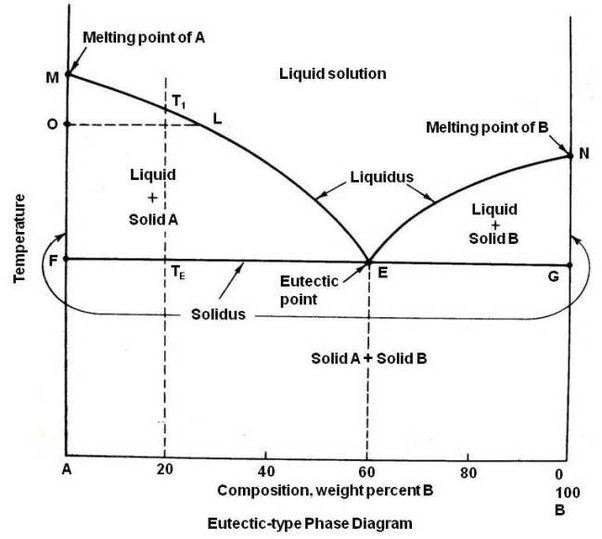
\includegraphics[width=\textwidth]{Diagrammi di fase/eutettico.jpg}
\end{minipage}

\begin{minipage}[b]{0.5\linewidth}
\centering
    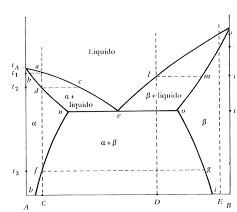
\includegraphics[width=\textwidth]{Diagrammi di fase/partial_solub.png}
\end{minipage}

\label{eutettico}
\caption{Sopra: diagramma di fase di un eutettico in una situazione di sostanze totalmente immiscibili. Sotto: diagramma di fase di un sistema a solubilità parziale.}
\end{figure}

A composizione diversa da quella eutettica si osserva una trasformazione di fase incoerente. Se ci troviamo oltre quella composizione avremo prima la formazione del cristallo B e poi la solidificazione dell'eutettico (caso \textbf{\textit{iper-eutettico}}), se invece ci troviamo prima otterremo prima la solidificazione di A e poi dell'eutettico (caso \textbf{\textit{ipoeutettico}}).
Al punto eutettico si possono osservare microstrutture di vario tipo:

\begin{itemize}
    \item \textbf{\textit{Lamellari}} o \textbf{\textit{Perliti}} in cui le microstrutture sono degli strati di fase differente.
    \item \textbf{\textit{Globulari}} dove si hanno dei cristalli sferici di una fase immersi nell'altra.
    \item \textbf{\textit{Dendritico}} dove si hanno cristalli sferici con all'interno domini lamellari.
    \item \textbf{\textit{Aciculare}} dove si hanno dei cristalli a forma di aghi immersi negli altri.
\end{itemize}

Al di fuori del punto eutettico si ha che ai bordi di grano inizia la cristallizzazione della fase a concentrazione maggiore.
Esistono altre transizioni di fase in base alle fasi iniziali e finali del processo. Queste fasi sono riportati in Fig \ref{three-phase-reactions}. Queste transizioni hanno in comune che durante la transizione la composizione non cambia e vengono detti \textbf{\textit{trasformazioni congruenti}}.
In genere a particolari valori di composizione (tali per cui si hanno rapporti interi nei numeri atomici) si possono avere dei \textbf{\textit{composti intermetallici}}, composti chimici a tutti gli effetti (ad esempio la cementite nel caso dell'acciaio).

\begin{figure}[h]
    \centering
    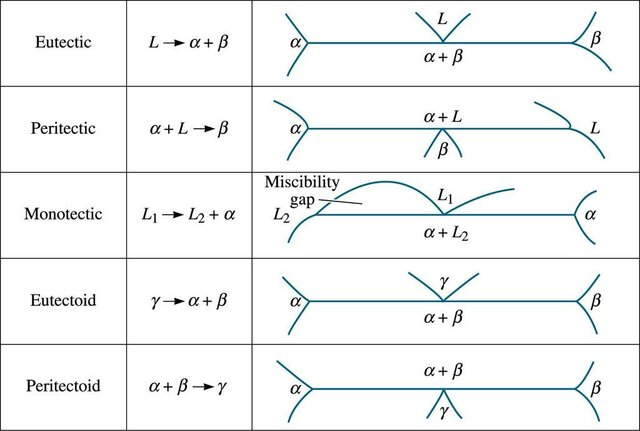
\includegraphics[width=10cm]{Diagrammi di fase/three-phase-reacctions.jpg}
    \caption{Three-phase transitions.}
    \label{three-phase-reactions}
\end{figure}